\section{Data Distribution Service}

DDS is a messaging middleware standard \cite{dds-1.4-standard} for distributed applications. The standard is designed for mission- and business critical systems with real-tme requirements. As such, it aims to function in a resource efficient and predictable manner, succumbing to minimal computational and transport overhead.

Specifies an API by which a distributed application can pass data over DCPS. 



DDS is built around the data-centric publish-subscribe paradigm.
Data centric means....

In the publish-subscribe paradigm, two kinds of peers are present: publishers and subscribers. Publishers offer data, while subscribers subscribe to receive that data. A crucial characteristic of publish-subscribe is that data exchange between the peers is anonymous. \Ie , subscribers do not know where a given message originated. The same is true for publishers: they have no knowledge about where the sent data will end up at -- or even if there are any receivers. Thus, there is no concept of \emph{direct addressing}. Instead, peers communicate on the basis of a shared understanding of what \emph{kind of data} they are interested in. 
For example, given a temperature sensor offering temperature measurements in a publish-subscribe setting. A subscriber that is interested in that data only knows that it wants to receive \emph{temperature data} while at the same time being entirely oblivious to the concept of \emph{temperature sensors}. 
Since publishers and subscribers have no references to one another, and know as little of each other as possible, a high level of loose coupling is achieved. This allows for a simple extension of the system, making it extraordinarily scalable.

By abstracting away the source of data, a \emph{virtual global data space} is created. Each component connected to the system views data as if it were available in a local storage, when in reality, it is distributed.


\paragraph{Programming Interface.}
The DDS specification is split into two separate sections. The main one, which is concerned with \emph{Data-Centric Publish-Subscribe} (DCPS), defines a low level API that enables applications to communicate via DDS. The second part revolves around a \emph{Data Local Reconstruction Layer} (DLRL). DLRL sits on top of DCPS and is optional. The purpose of DLRL is to provide typed interfaces to the messaging layer, \ie , the delivered messages are conceived in a format suitable for direct processing in the application--without the need to check the message's format. More precisely, DCPS performs a transformation of the unprocessed messages into language-specific data types. With the aid of DLRL, type-safety of communication is ensured and verification can be performed at compile-time, thereby reducing the application's error-proneness.


\paragraph{Wire Protocol.}
At the base of DDS, there is a wire protocol deliberately tailored to DCPS-style communication: Real-time Publish-Subscribe (RTPS). Although RTPS is related to DDS, its specifics are outsourced in a separate standard. \cite{rtps-2.2-standard}

Goals: provide platform independent means of communication to make DDS implementations interoperable.



\paragraph{Bla}
Offers transport transparency.

data-centric instead of message-centric. The difference is that the former implies a shared data model. The middleware has an understanding of the data and its context and is responsible that all components have a common view of the data.
The advantage of data-centric messaging is that it allows a higher abstraction. Developers can focus on the data itself and on developing business logic instead of having to implement data sharing through exchange of messages.

DDS is a message bus. This is in contrast to a broker-based architecture. A broker enables flexible routing patterns featuring filtering, variable numbers of message queues etc. However, it can be considered a single point of failure.

Being a standard, DDS strives for interoperability between implementations


\begin{figure}[htpb]
  \centering
  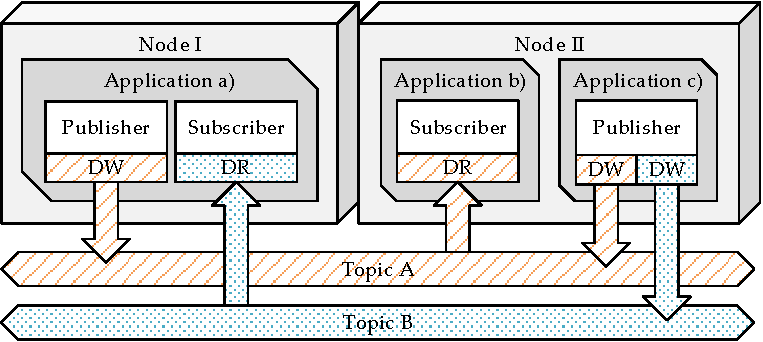
\includegraphics[width=\textwidth]{figures/dds.pdf}
  \caption[DDS example]{An example of a distributed application connected by means of DDS}\label{fig:dds}
\end{figure}

\subsection{DDS Components}

DDS defines a number of components, for which it uses its own nomenclature. In the following, each component is described. \autoref{fig:dds} shows how they are related.


\paragraph{Topics.}


\paragraph{Publishers and Data Writers.}


\paragraph{Subscribers and Data Readers.}

\paragraph{Domains and Domain Participants.}
At the highest level, there are \emph{Domains}. Domains are the DDS way of grouping together sets of coherent \emph{domain participants} and to separate those sets from each other. Speaking in terms of distributed systems, domains are a mechanism to manage group memberships of nodes. \cite{tanenbaum2017distributed}

Domain participants are entities that belong to a particular domain. Each publisher, subscriber and topic is derived from one domain participant and is therefore dedicated to exactly that domain. As a consequence, participants of different domains are entirely separated from each other.   

Depicted in \autoref{fig:dds} is only one domain. However, there could just as well be other domains. 



\subsection{Concepts}

\paragraph{Data Centricity.}


\paragraph{Dynamic Service Discovery.}
Offers dynamic service discovery.


\paragraph{Quality of Service.}
One of DDS's salient features is its intrinsic QoS support implemented by \emph{QoS policies}.
QoS policies specify service attributes for controlling each participant's behavior and quality properties. They can be set for each participant and topic individually. An example for a QoS policy is the \texttt{DEADLINE} policy. It specifies the minimum message frequency of a service. If the deadline period of a hypothetical data writer is set to, e.g., 100 ms, that means that this data writer is required to send a message at least every 100 ms. If it fails to send a message at this rate, the data writer and all the respective topic's readers will need to deal with this circumstance on a code level. 

In addition, QoS policies serve as service contracts. They specify non-functional requirements that services must fulfill to be able to communicate with each other. E.g., a service provider's \texttt{RELIABILITY} policy may have been set to the \texttt{BEST\_EFFORT} level, thereby allowing the service to drop samples. A service consumer, on the other hand, may require the service provider's policy to be set to \texttt{RELIABLE}, which prohibits the dropping of samples. Since the service provider only insufficiently fulfills the service consumer's QoS requirements, the services are considered incompatible with each other. QoS policies can therefore be seen as service contracts on a technical level, specifying service compatibility. It may be noteworthy, however, that these contracts do not rid the need for proper interface contracts modeled by a service designer.

Despite their name, QoS policies do not only concern quality attributes. They can also be used to specify the priority of messages, their lifespan, i.e. how long they are valid, or how many messages are kept in local memory.



\paragraph{Data Centricity.}

\paragraph{Asynchronous Messaging.}


\paragraph{Location Transparency.}

\paragraph{Decentralization.}

\paragraph{Platform Independence.}


\paragraph{Limitations.}
Requires full fledged operating system which can not be guaranteed in embedded systems.

OpenDDS: Up to 120 domain participants


\subsection{DDS for Automotive Systems}
Automotive software systems have previously relied -- and, to some degree, will continue to do so -- on low-level, low-bandwidth transport protocols such as CAN, LIN, FlexRay, etc. Up until now, networks stacks based on those protocols were sufficient to meet the basic requirements of delivering vehicular sensor data. However, in the future, more and more data will be collected within vehicles and more and more data will be required to feed into intelligent systems such as ADAS. These systems increasingly rely on high volumes of data from video cameras, or LIDARs. As a result, bandwidth requirements for vehicle-intrinsic computer networks are skyrocketing. At the same time, these functions require computational capabilities that go way beyond of what is possible with the microcontrollers typically used in traditional ECUs. High-performance computer systems based on high-level operating systems are needed to meet the new requirements.


Hence, there is a need for 

DDS is designed for resource constrained real-time applications such as sensor networks or industrial automation.

DDS allows to configure how much of a system's resources an DDS-enabled application may use. Consequently, it is the middleware's responsibility to allocate resources as needed while still staying within the specified boundaries. At the same time, priorities aligning with the application's QoS settings need to be considered. DDS takes this burden off the programmer's shoulders.

Predictable


\subsection{Implementations}
As mentioned, DDS, in itself, is only a standard. As such, DDS does not dictate, in detail, how to implement the concepts presented in the earlier sections. A number of DDS implementations by different vendors exist, all varying in terms of standard fulfillment, features beyond the standard, and pricing. Compatibility between the respective implementations is ensured through the \emph{DDS Interoperability Protocol} (DDSI). It uses the OMG \emph{Common Data Representation} (CDR) to encode data in a platform-neutral way. 

\paragraph{OpenDDS.}
Two types of discovery: centralized Information Repository, distributed RTPS discovery. The latter must be used if DDS implementation compatibility is priority

Only supports C++ and Java

\paragraph{OpenSplice.}


\paragraph{RTI.}
out of the implementations available to the broad public, it is by far the most mature and feature rich implementation.
Features encryption, compliance to several safety standards

\paragraph{Others.}
Miltech